

\tikzset{every picture/.style={line width=0.75pt}} %set default line width to 0.75pt        

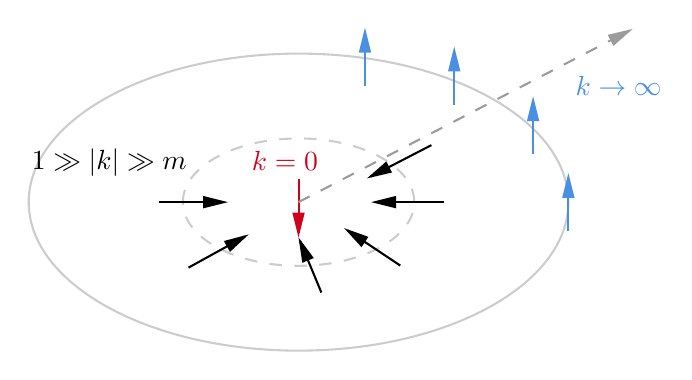
\begin{tikzpicture}[x=0.75pt,y=0.75pt,yscale=-1,xscale=1]
%uncomment if require: \path (0,300); %set diagram left start at 0, and has height of 300

%Shape: Ellipse [id:dp6127707106898874] 
\draw  [color={rgb, 255:red, 0; green, 0; blue, 0 }  ,draw opacity=0.2 ] (100,183.56) .. controls (100,144.04) and (158.2,112) .. (230,112) .. controls (301.8,112) and (360,144.04) .. (360,183.56) .. controls (360,223.08) and (301.8,255.11) .. (230,255.11) .. controls (158.2,255.11) and (100,223.08) .. (100,183.56) -- cycle ;
%Straight Lines [id:da5498048117239558] 
\draw [color={rgb, 255:red, 208; green, 2; blue, 27 }  ,draw opacity=1 ]   (230,172.56) -- (230,198.56) ;
\draw [shift={(230,200.56)}, rotate = 270] [fill={rgb, 255:red, 208; green, 2; blue, 27 }  ,fill opacity=1 ][line width=0.08]  [draw opacity=0] (12,-3) -- (0,0) -- (12,3) -- cycle    ;
%Straight Lines [id:da8202921841687136] 
\draw [color={rgb, 255:red, 74; green, 144; blue, 226 }  ,draw opacity=1 ]   (360,197.56) -- (360,171.56) ;
\draw [shift={(360,169.56)}, rotate = 90] [fill={rgb, 255:red, 74; green, 144; blue, 226 }  ,fill opacity=1 ][line width=0.08]  [draw opacity=0] (12,-3) -- (0,0) -- (12,3) -- cycle    ;
%Straight Lines [id:da9640331300182798] 
\draw [color={rgb, 255:red, 74; green, 144; blue, 226 }  ,draw opacity=1 ]   (343,160.56) -- (343,134.56) ;
\draw [shift={(343,132.56)}, rotate = 90] [fill={rgb, 255:red, 74; green, 144; blue, 226 }  ,fill opacity=1 ][line width=0.08]  [draw opacity=0] (12,-3) -- (0,0) -- (12,3) -- cycle    ;
%Straight Lines [id:da03242442582564298] 
\draw [color={rgb, 255:red, 74; green, 144; blue, 226 }  ,draw opacity=1 ]   (305,136.56) -- (305,110.56) ;
\draw [shift={(305,108.56)}, rotate = 90] [fill={rgb, 255:red, 74; green, 144; blue, 226 }  ,fill opacity=1 ][line width=0.08]  [draw opacity=0] (12,-3) -- (0,0) -- (12,3) -- cycle    ;
%Straight Lines [id:da22373788973980524] 
\draw [color={rgb, 255:red, 74; green, 144; blue, 226 }  ,draw opacity=1 ]   (262,127.56) -- (262,101.56) ;
\draw [shift={(262,99.56)}, rotate = 90] [fill={rgb, 255:red, 74; green, 144; blue, 226 }  ,fill opacity=1 ][line width=0.08]  [draw opacity=0] (12,-3) -- (0,0) -- (12,3) -- cycle    ;
%Straight Lines [id:da7619994864927513] 
\draw [color={rgb, 255:red, 155; green, 155; blue, 155 }  ,draw opacity=1 ] [dash pattern={on 4.5pt off 4.5pt}]  (230,183.56) -- (389.22,101.03) ;
\draw [shift={(391,100.11)}, rotate = 152.6] [fill={rgb, 255:red, 155; green, 155; blue, 155 }  ,fill opacity=1 ][line width=0.08]  [draw opacity=0] (12,-3) -- (0,0) -- (12,3) -- cycle    ;
%Shape: Ellipse [id:dp3388918869189159] 
\draw  [color={rgb, 255:red, 0; green, 0; blue, 0 }  ,draw opacity=0.2 ][dash pattern={on 4.5pt off 4.5pt}] (174.25,183.56) .. controls (174.25,166.61) and (199.21,152.87) .. (230,152.87) .. controls (260.79,152.87) and (285.75,166.61) .. (285.75,183.56) .. controls (285.75,200.51) and (260.79,214.24) .. (230,214.24) .. controls (199.21,214.24) and (174.25,200.51) .. (174.25,183.56) -- cycle ;
%Straight Lines [id:da5105977529379926] 
\draw [color={rgb, 255:red, 0; green, 0; blue, 0 }  ,draw opacity=1 ]   (300,183.56) -- (267,183.56) ;
\draw [shift={(265,183.56)}, rotate = 360] [fill={rgb, 255:red, 0; green, 0; blue, 0 }  ,fill opacity=1 ][line width=0.08]  [draw opacity=0] (12,-3) -- (0,0) -- (12,3) -- cycle    ;
%Straight Lines [id:da00855087001959598] 
\draw [color={rgb, 255:red, 0; green, 0; blue, 0 }  ,draw opacity=1 ]   (163,183.56) -- (194,183.56) ;
\draw [shift={(196,183.56)}, rotate = 180] [fill={rgb, 255:red, 0; green, 0; blue, 0 }  ,fill opacity=1 ][line width=0.08]  [draw opacity=0] (12,-3) -- (0,0) -- (12,3) -- cycle    ;
%Straight Lines [id:da24612971832884312] 
\draw [color={rgb, 255:red, 0; green, 0; blue, 0 }  ,draw opacity=1 ]   (294,156.11) -- (264.78,171.2) ;
\draw [shift={(263,172.11)}, rotate = 332.7] [fill={rgb, 255:red, 0; green, 0; blue, 0 }  ,fill opacity=1 ][line width=0.08]  [draw opacity=0] (12,-3) -- (0,0) -- (12,3) -- cycle    ;
%Straight Lines [id:da6500494018973344] 
\draw [color={rgb, 255:red, 0; green, 0; blue, 0 }  ,draw opacity=1 ]   (177,215.11) -- (204.25,200.08) ;
\draw [shift={(206,199.11)}, rotate = 151.11] [fill={rgb, 255:red, 0; green, 0; blue, 0 }  ,fill opacity=1 ][line width=0.08]  [draw opacity=0] (12,-3) -- (0,0) -- (12,3) -- cycle    ;
%Straight Lines [id:da5631657523776881] 
\draw [color={rgb, 255:red, 0; green, 0; blue, 0 }  ,draw opacity=1 ]   (279,214.11) -- (253.66,197.22) ;
\draw [shift={(252,196.11)}, rotate = 33.69] [fill={rgb, 255:red, 0; green, 0; blue, 0 }  ,fill opacity=1 ][line width=0.08]  [draw opacity=0] (12,-3) -- (0,0) -- (12,3) -- cycle    ;
%Straight Lines [id:da5663091296229177] 
\draw [color={rgb, 255:red, 0; green, 0; blue, 0 }  ,draw opacity=1 ]   (241,227.11) -- (230.77,202.41) ;
\draw [shift={(230,200.56)}, rotate = 67.5] [fill={rgb, 255:red, 0; green, 0; blue, 0 }  ,fill opacity=1 ][line width=0.08]  [draw opacity=0] (12,-3) -- (0,0) -- (12,3) -- cycle    ;

% Text Node
\draw (362,121.4) node [anchor=north west][inner sep=0.75pt]  [color={rgb, 255:red, 74; green, 144; blue, 226 }  ,opacity=1 ]  {$\boldsymbol{k}\rightarrow \infty $};
% Text Node
\draw (206,157.4) node [anchor=north west][inner sep=0.75pt]  [color={rgb, 255:red, 208; green, 2; blue, 27 }  ,opacity=1 ]  {$\boldsymbol{k} =0$};
% Text Node
\draw (100,156.4) node [anchor=north west][inner sep=0.75pt]    {$1\gg |\boldsymbol{k} |\gg m$};


\end{tikzpicture}
